% Options for packages loaded elsewhere
\PassOptionsToPackage{unicode}{hyperref}
\PassOptionsToPackage{hyphens}{url}
\PassOptionsToPackage{dvipsnames,svgnames,x11names}{xcolor}
%
\documentclass[
  ignorenonframetext,
]{beamer}
\usepackage{pgfpages}
\setbeamertemplate{caption}[numbered]
\setbeamertemplate{caption label separator}{: }
\setbeamercolor{caption name}{fg=normal text.fg}
\beamertemplatenavigationsymbolsempty
% Prevent slide breaks in the middle of a paragraph
\widowpenalties 1 10000
\raggedbottom
\setbeamertemplate{part page}{
  \centering
  \begin{beamercolorbox}[sep=16pt,center]{part title}
    \usebeamerfont{part title}\insertpart\par
  \end{beamercolorbox}
}
\setbeamertemplate{section page}{
  \centering
  \begin{beamercolorbox}[sep=12pt,center]{part title}
    \usebeamerfont{section title}\insertsection\par
  \end{beamercolorbox}
}
\setbeamertemplate{subsection page}{
  \centering
  \begin{beamercolorbox}[sep=8pt,center]{part title}
    \usebeamerfont{subsection title}\insertsubsection\par
  \end{beamercolorbox}
}
\AtBeginPart{
  \frame{\partpage}
}
\AtBeginSection{
  \ifbibliography
  \else
    \frame{\sectionpage}
  \fi
}
\AtBeginSubsection{
  \frame{\subsectionpage}
}
\usepackage{amsmath,amssymb}
\usepackage{iftex}
\ifPDFTeX
  \usepackage[T1]{fontenc}
  \usepackage[utf8]{inputenc}
  \usepackage{textcomp} % provide euro and other symbols
\else % if luatex or xetex
  \usepackage{unicode-math} % this also loads fontspec
  \defaultfontfeatures{Scale=MatchLowercase}
  \defaultfontfeatures[\rmfamily]{Ligatures=TeX,Scale=1}
\fi
\usepackage{lmodern}
\ifPDFTeX\else
  % xetex/luatex font selection
\fi
% Use upquote if available, for straight quotes in verbatim environments
\IfFileExists{upquote.sty}{\usepackage{upquote}}{}
\IfFileExists{microtype.sty}{% use microtype if available
  \usepackage[]{microtype}
  \UseMicrotypeSet[protrusion]{basicmath} % disable protrusion for tt fonts
}{}
\makeatletter
\@ifundefined{KOMAClassName}{% if non-KOMA class
  \IfFileExists{parskip.sty}{%
    \usepackage{parskip}
  }{% else
    \setlength{\parindent}{0pt}
    \setlength{\parskip}{6pt plus 2pt minus 1pt}}
}{% if KOMA class
  \KOMAoptions{parskip=half}}
\makeatother
\usepackage{xcolor}
\newif\ifbibliography
\usepackage{graphicx}
\makeatletter
\def\maxwidth{\ifdim\Gin@nat@width>\linewidth\linewidth\else\Gin@nat@width\fi}
\def\maxheight{\ifdim\Gin@nat@height>\textheight\textheight\else\Gin@nat@height\fi}
\makeatother
% Scale images if necessary, so that they will not overflow the page
% margins by default, and it is still possible to overwrite the defaults
% using explicit options in \includegraphics[width, height, ...]{}
\setkeys{Gin}{width=\maxwidth,height=\maxheight,keepaspectratio}
% Set default figure placement to htbp
\makeatletter
\def\fps@figure{htbp}
\makeatother
\setlength{\emergencystretch}{3em} % prevent overfull lines
\providecommand{\tightlist}{%
  \setlength{\itemsep}{0pt}\setlength{\parskip}{0pt}}
\setcounter{secnumdepth}{-\maxdimen} % remove section numbering
% mystyle3.tex
\usepackage{graphicx}
\titlegraphic{
    
\includegraphics[height=1.5cm]{UniUrb-logo.png}\hfill
    
\includegraphics[height=1.5cm]{bremen_logo.png}
}

 \definecolor{myblue}{HTML}{005997}
  \setbeamercolor{frametitle}{fg=myblue}
    \setbeamercolor{framesubtitle}{fg=myblue}
    \setbeamercolor{frametitle right}{fg=myblue}
  \setbeamercolor{titlelike}{fg=myblue}
    \setbeamercolor{title}{fg=myblue}
      \setbeamercolor{subtitle}{fg=myblue}
    \setbeamercolor{part title}{fg=myblue}
    \setbeamercolor{section title}{fg=myblue}
    \setbeamercolor{subsection title}{fg=myblue}
  \setbeamercolor{section name}{fg=myblue}
  \setbeamercolor{subsection name}{fg=myblue}
  \setbeamercolor{part name}{fg=myblue}
  \setbeamercolor{title in head/foot}{fg=myblue}
  \setbeamercolor{subtitle in head/foot}{fg=myblue}
  \setbeamercolor{block title}{fg=myblue}
  
  \setbeamercolor{bullet}{fg=myblue}
  \setbeamercolor{section in toc}{fg=myblue}
  \setbeamercolor{subsection in toc}{fg=myblue}
  \setbeamercolor{section in head/foot}{fg=myblue}
  \setbeamercolor{subsection in head/foot}{fg=myblue}
  
  
  \setbeamercolor{itemize item}{fg = myblue}
  \setbeamercolor{itemize subitem}{fg = myblue}
  \setbeamercolor{itemize subsubitem}{fg = myblue}
  \setbeamercolor{enumerate item}{fg = myblue}
  \setbeamercolor{enumerate subitem}{fg = myblue}
  \setbeamercolor{enumerate subsubitem}{fg = myblue}
\usepackage{etoolbox}
\AtBeginEnvironment{thebibliography}{\scriptsize}
\ifLuaTeX
  \usepackage{selnolig}  % disable illegal ligatures
\fi
\usepackage[round]{natbib}
\bibliographystyle{plainnat}
\usepackage{bookmark}
\IfFileExists{xurl.sty}{\usepackage{xurl}}{} % add URL line breaks if available
\urlstyle{same}
\hypersetup{
  pdftitle={Tracking the Digital Divide: Factor Analysis and Time Trends in Italian Firms},
  pdfauthor={Luis Carlos Castillo},
  colorlinks=true,
  linkcolor={myblue},
  filecolor={Maroon},
  citecolor={Blue},
  urlcolor={Blue},
  pdfcreator={LaTeX via pandoc}}

\title{Tracking the Digital Divide: Factor Analysis and Time Trends in
Italian Firms}
\author{Luis Carlos Castillo}
\date{02 July 2024}
\institute{Binational Doctorate\\
University of Urbino and Universty of Bremen\\
Ph.D.~Program in Global Studies\\
Supervisor: Prof.~Francesco Vidoli\\
Co-Supervisor: Prof.~Dr.~Christian Cordes}

\begin{document}
\frame{\titlepage}

\begin{frame}{Cumulative Dissertation}
\phantomsection\label{cumulative-dissertation}
\begin{center}
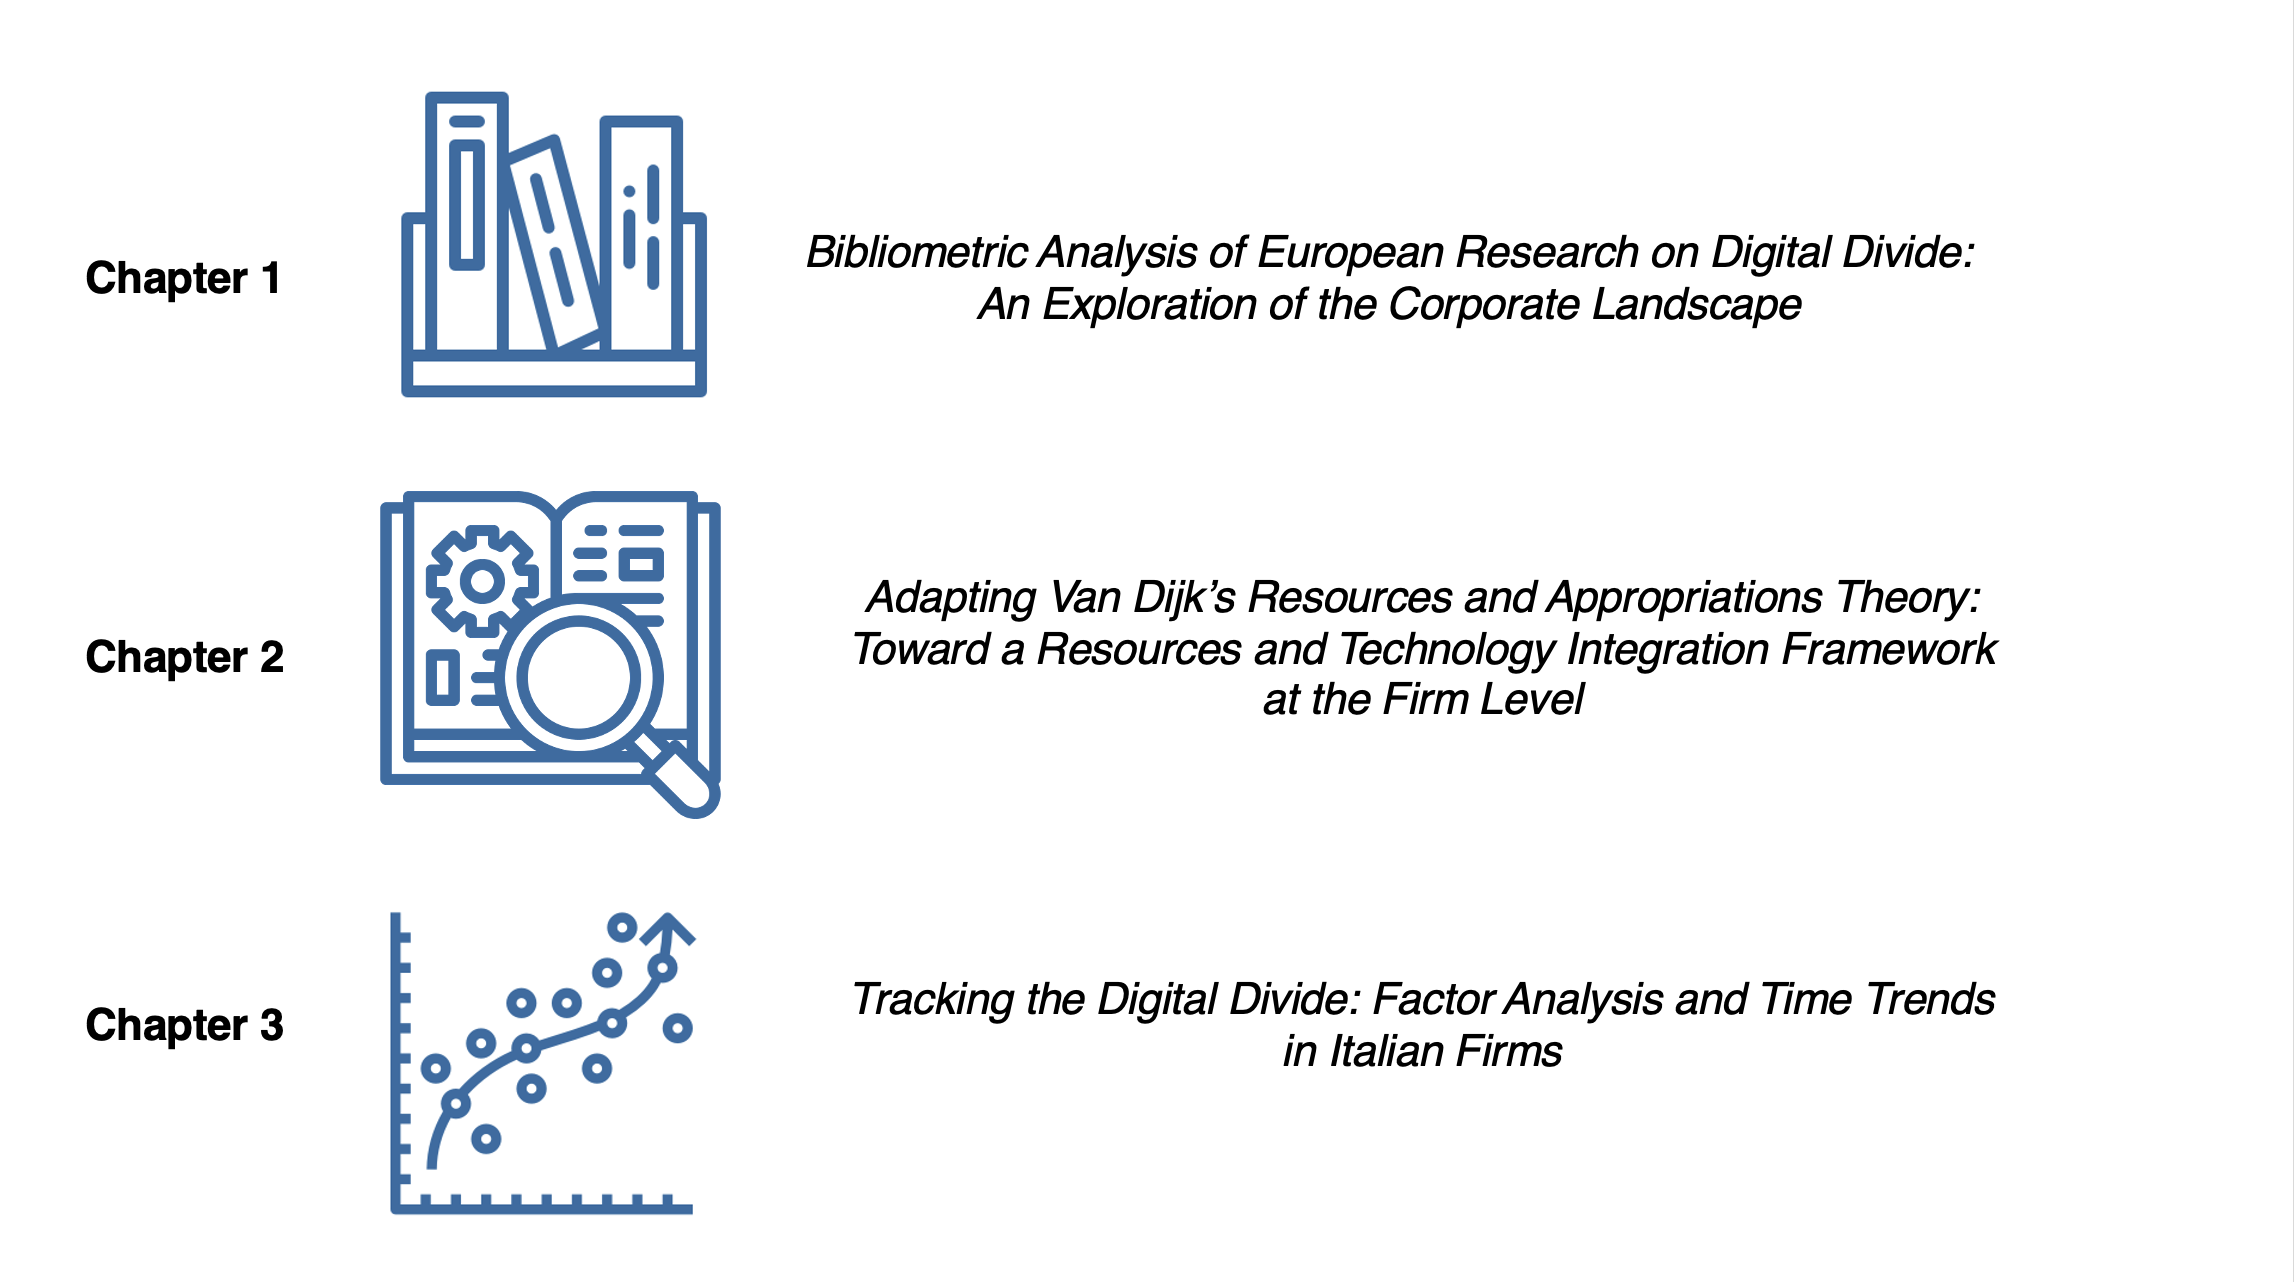
\includegraphics[width=1.1\textwidth, height=1.2\textheight]{structure_thesis1.png}
\end{center}
\end{frame}

\begin{frame}{1. Introduction}
\phantomsection\label{introduction}
\begin{itemize}
\item
  DT play a pivotal role in reshaping business models
  \citep{trischler2023} , driving innovation \citep{ciarli2021}, and
  fostering competitive advantages \citep{jeganjosephjerome2024}.
\item
  The unequal adoption of DT has led to significant challenge: the
  digital divide.
\item
  The digital divide at the firm level is a multifaceted gap
  characterized not only by disparities in access, skills and usage of
  DT, but also the derived benefits from different types of use.
\item
  While the digital divide is a global issue, its impact on enterprises,
  especially in Italy, presents unique challenges and opportunities.
\end{itemize}
\end{frame}

\begin{frame}{2. Objectives}
\phantomsection\label{objectives}
\begin{itemize}
\item
  Explore changes over time in the digital divide, focusing on
  differences across firm sizes, sectors, and regions.
\item
  Develop composite indices to track trends in the first and
  second-level digital divide.
\item
  Evaluate the alignment of resources and technology integration theory
  with observed data.
\item
  Propose targeted policy interventions based on research findings.
\end{itemize}
\end{frame}

\begin{frame}{3. Data}
\phantomsection\label{data}
\begin{itemize}
\item
  The dataset was derived from the ICT Usage in Enterprises Survey
  conducted annually between 2014 and 2019 by ISTAT.
\item
  In total, 29 variables were used to extract three factors that
  represent the theoretical constructs.

  \begin{itemize}
  \tightlist
  \item
    Access index: 6 variables
  \item
    Skills index: 9 variables
  \item
    Usage index: 11 variables
  \item
    \textbf{Control variable:} Firm size with three categories (small,
    medium, large)
  \end{itemize}
\item
  Considerations and Limitations.

  \begin{itemize}
  \tightlist
  \item
    Independence of Annual Data
  \end{itemize}
\item
  Data treatments, codes, and summary statistics, are available on my
  \href{https://github.com/luchocastillo84/Factor_Analysis_Digital_Divide/tree/main}{GitHub
  repository} for replicability and further analysis.
\end{itemize}
\end{frame}

\begin{frame}{4. Methodology}
\phantomsection\label{methodology}
\begin{itemize}
\tightlist
\item
  The indices were constructed using dimensionality reduction techniques
  Factor Analysis for Mixed Data (FAMD) and Multiple Correspondence
  Analysis (MCA).
\end{itemize}

\[ \text{Access Index}_i = \sum_{j=1}^{6} a_j \cdot X_{j,i} \cdot w_i \]
\[ \text{Skills Index}_i = \sum_{k=1}^{9} b_k \cdot Y_{k,i} \cdot w_i \]
\[ \text{Usage Index}_i = \sum_{m=1}^{11} c_m \cdot Z_{m,i} \cdot w_i \]

Where \(\mathbf{X}\), \(\mathbf{Y}\), and \(\mathbf{Z}\) are the
matrices of observations, \(\mathbf{a}\), \(\mathbf{b}\), and
\(\mathbf{c}\) are the vectors of weights derived from FAMD and MCA
contributions of each variable to the retained dimensions, and
\(\mathbf{w}\) is the vector of weights accounting for the share of
groups and years.

\[ \text{Access Index}_i = \sum_{j=1}^{6} a_j \cdot X_{j,i} \]
\[ \text{Skills Index}_i = \sum_{k=1}^{9} b_k \cdot Y_{k,i} \]
\[ \text{Usage Index}_i = \sum_{m=1}^{11} c_m \cdot Z_{m,i} \]
\end{frame}

\begin{frame}{5. Results I}
\phantomsection\label{results-i}
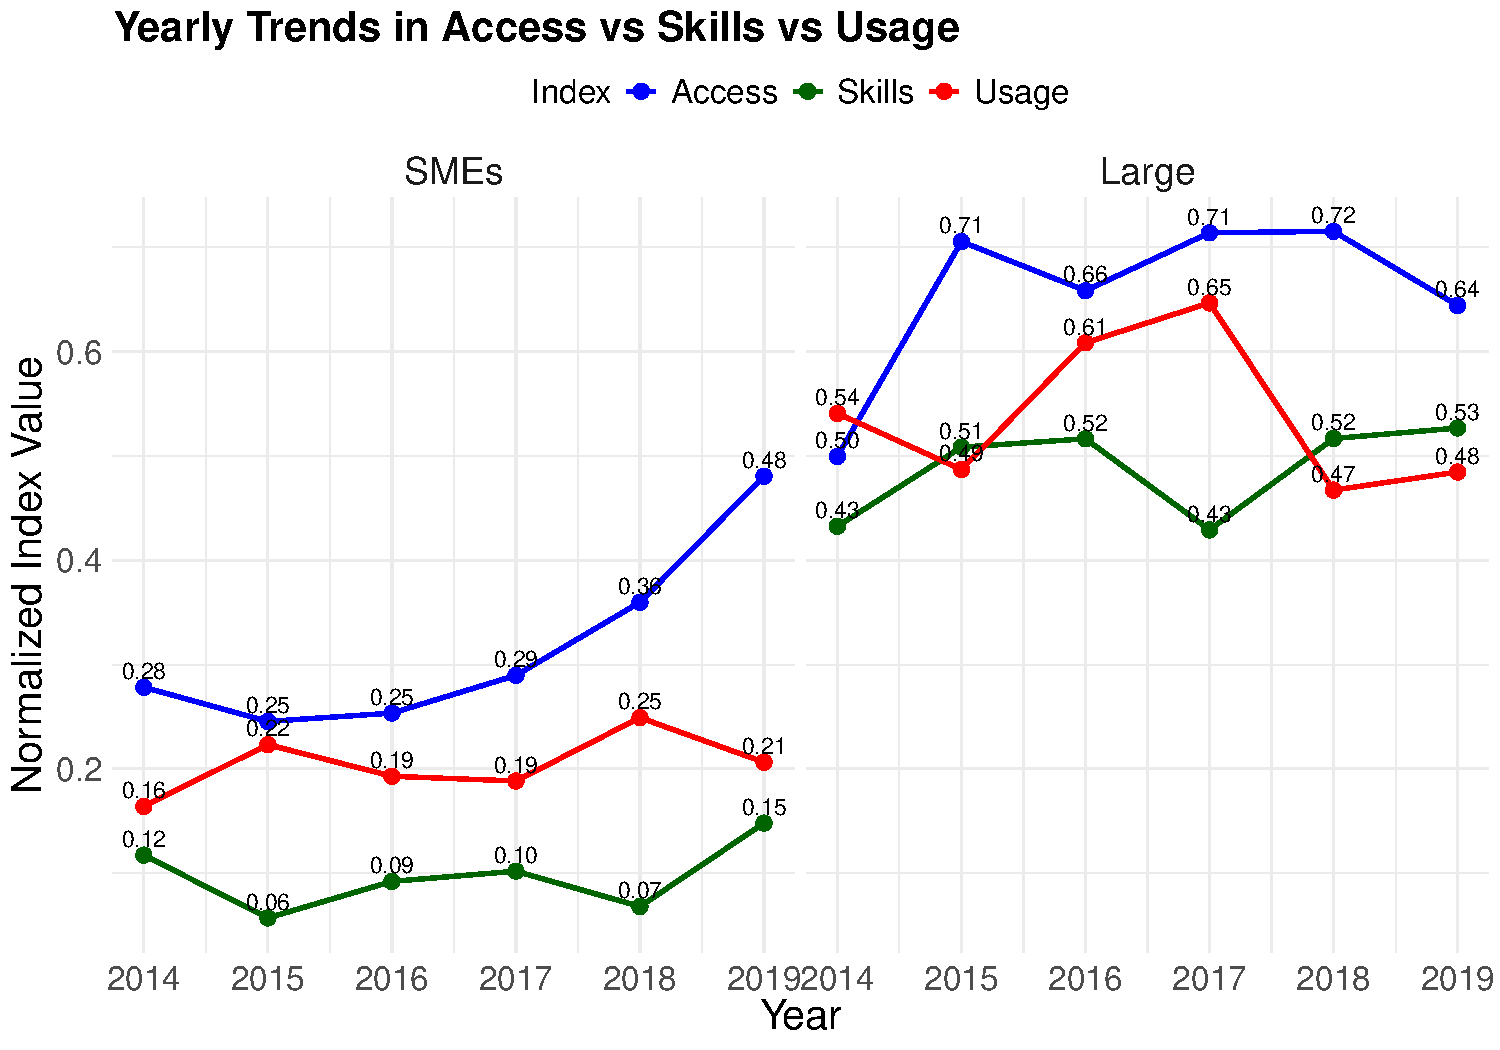
\includegraphics{FactoAnalysisDigitalDivide_files/figure-beamer/yearTrendSize-1.pdf}
\end{frame}

\begin{frame}{Key takeaways I}
\phantomsection\label{key-takeaways-i}
\begin{itemize}
\item
  While SMEs can maintain continuous growth in access, larger firms face
  different challenges.
\item
  These findings align with Bratta et al.~(2020), who discuss the
  hyper-depreciation measure issued in 2016.
\item
  SMEs face more challenges in acquiring digital skills. There is a
  significant shortage of ICT graduates in Italy according to the
  ``Digital Skills Observatory'' in 2019.
\item
  A higher usage index is present in SMEs as existing technologies need
  to be operated either by outsourcing digital skills or maximising the
  existing workforce.
\end{itemize}
\end{frame}

\begin{frame}{5.1. Results II}
\phantomsection\label{results-ii}
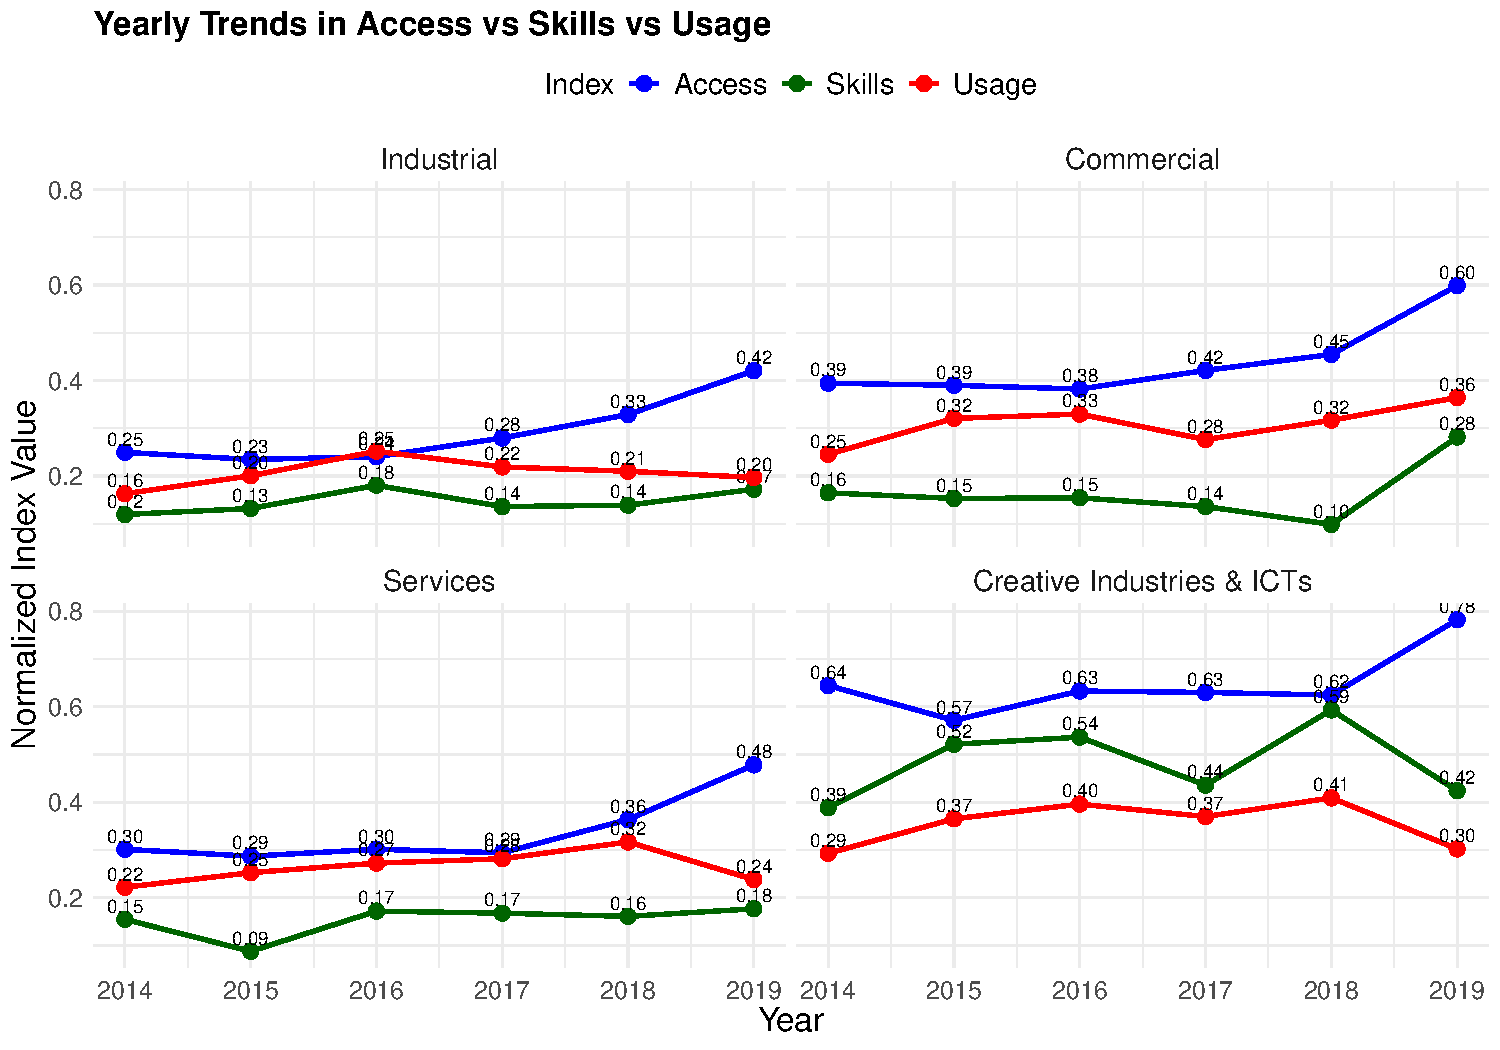
\includegraphics{FactoAnalysisDigitalDivide_files/figure-beamer/yearTrendMac-1.pdf}
\end{frame}

\begin{frame}{Key takeaways II}
\phantomsection\label{key-takeaways-ii}
\begin{itemize}
\item
  Notable progress in digital access across sectors due to effective
  policy measures like hyper-depreciation.
\item
  The digital skills index remains low, highlighting challenges in
  developing necessary competencies.
\item
  Commercial, Industrial, Service Sectors: Growing digital access and
  stable usage, but significant skills gap.
\item
  Creative Industries and ICT Sector: High levels of access and skills
  but moderate usage, reflecting different technological needs in
  workflows.
\end{itemize}
\end{frame}

\begin{frame}{5.2. Results III}
\phantomsection\label{results-iii}
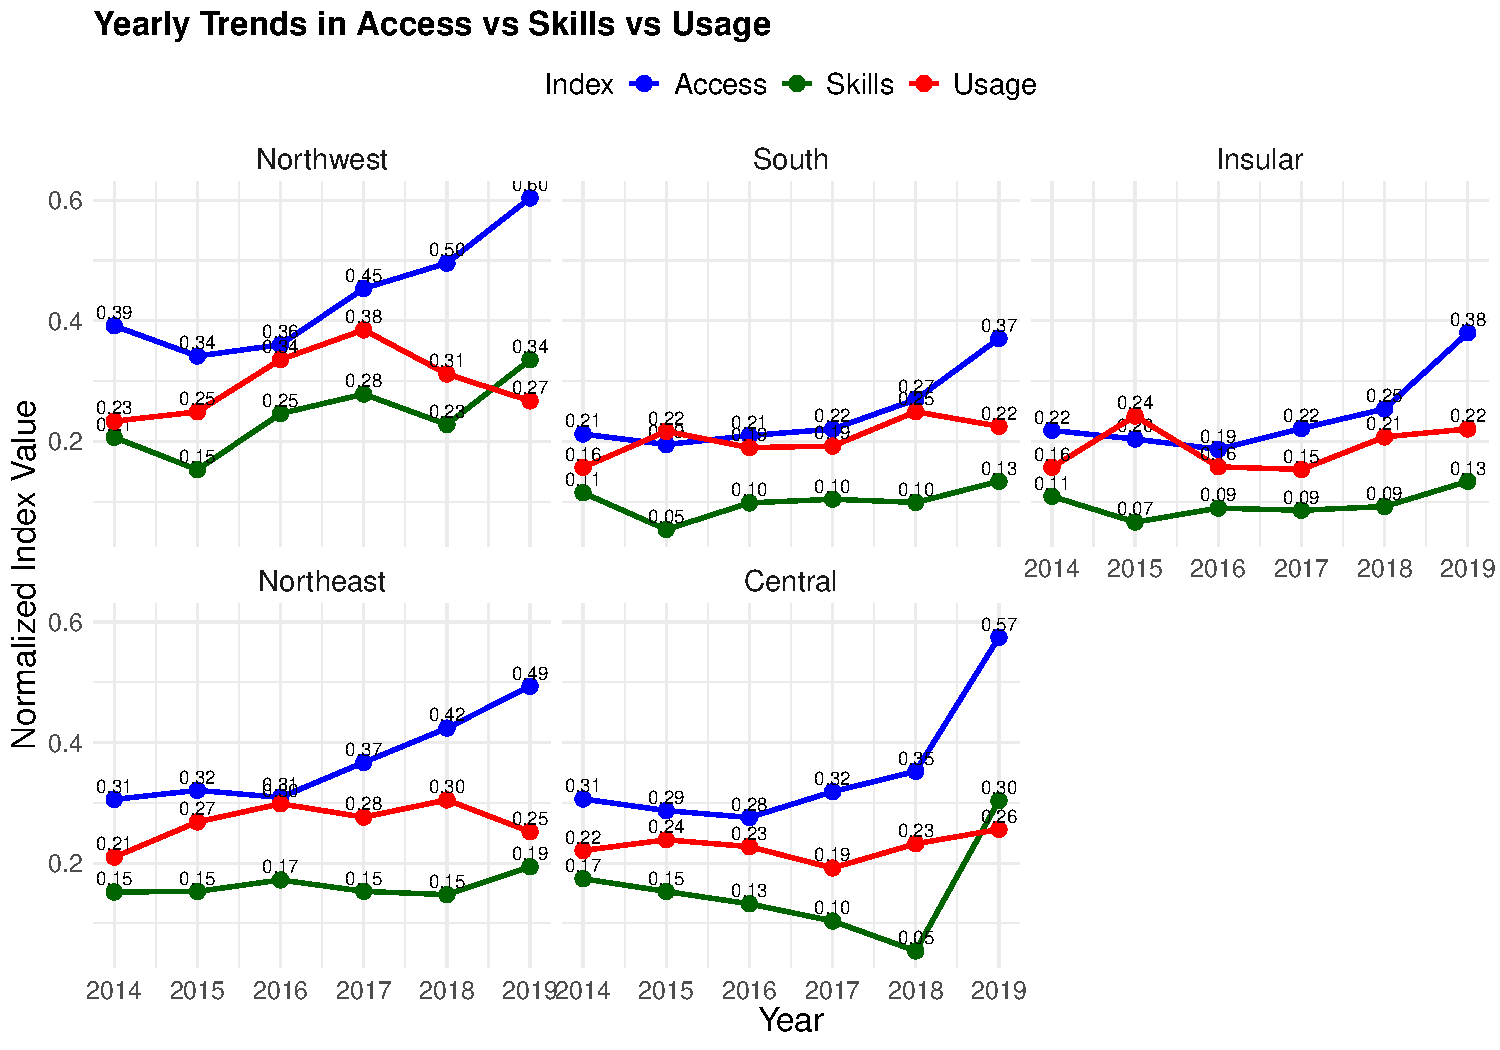
\includegraphics{FactoAnalysisDigitalDivide_files/figure-beamer/yearTrendReg-1.pdf}
\end{frame}

\begin{frame}{Key takeaways III}
\phantomsection\label{key-takeaways-iii}
\begin{itemize}
\item
  Northern and Central Regions:

  \begin{itemize}
  \tightlist
  \item
    Significant improvements in digital access.
  \item
    Benefits from robust industrial bases and policy interventions.
  \item
    Persistent skills gap, slight increase towards the end.
  \end{itemize}
\item
  South and Insular Regions:

  \begin{itemize}
  \tightlist
  \item
    Lag behind in both access and skills. Reflecting systemic issues.
  \item
    Need targeted policy efforts.
  \end{itemize}
\item
  Usage Trends:

  \begin{itemize}
  \tightlist
  \item
    Similar trends across regions.
  \item
    DT integration driven by national policies, market forces, and
    sectoral requirements.
  \end{itemize}
\end{itemize}
\end{frame}

\begin{frame}{6. Q\&A}
\phantomsection\label{qa}
Thank you for your attention
\end{frame}

\renewcommand\refname{References}
\begin{frame}[allowframebreaks]{References}
  \bibliographytrue
  \bibliography{ShiftPatterns.bib}
\end{frame}

\end{document}
